\header{
    \section{Jaune} \label{jaune}
    %
    \insertComment{Chanson de 34Alain34 le 19/12/2011}{}
}

\enluminure{4}{\href{https://www.youtube.com/watch?v=wNch1OqYgIM}{J}}{aune,} comme un ricard servi avant d'aller manger
\\Jaune, avé deux trois glaçons au fond d'un verre à pied
\\Jaune et deux volumes d'eau, je l'aime bien tassé !
\\Jaune, avé quelques olives pour bien l'accompagner
\\Jaune, avé deux trois copains la convivialité
\\Jaune, pour refaire le monde quand je suis bien pété
\\Jaune, je l'aime tellement c'est mon petit péché
\\Jaune en trempant des croissants au petit déjeuner
\\\\\textbf{Refrain :}
\\J'en bois à l'apéro, c'est bon c'est anisé
\\J'en bois aussi au digeot, c'est pas bon mélangé
\\J'en bois entre les repas pour me désaltérer
\\Je vide les bouteilles parfois c'est abusé
\\\\Jaune, comme le feu des gitans autour des poulaillers
\\Jaune, comme le maillot d'Indurain sur les Champs-Élysées
\\Jaune, comme l'auto de la poste qu'amène le courrier
\\Jaune, comme le blanc de mes yeux quand je suis défoncé
\\\\Jaune, comme un ricard servit avant d'aller manger
\\Jaune, avé deux trois glaçons au fond d'un verre à pied
\\Jaune et deux volumes d'eau, je l'aime bien tassé
\\Jaune avé quelques olives pour bien l'accompagner
\\Jaune avé deux trois copains la convivialité
\\Jaune pour refaire le monde quand je suis bien pété
\\Jaune je l'aime tellement c'est mon petit péché
\\Jaune en trempant des croissants au petit déjeuner
\\\\Jaune, comme le feu des gitans autour des poulaillers
\\Jaune, comme le maillot d'Indurain sur les Champs-Élysées
\\Jaune, comme l'auto de la poste qu'amène le courrier
\\Jaune, comme le blanc de mes yeux quand je suis défoncé
\\\\\textbf{Refrain final :}
\\J'en bois à l'apéro, c'est bon c'est anisé
\\LALALLALALALLALALA
\\LALALALLALALALLALA
\\Je vide les bouteilles parfois c'est abusé
\bigskip
\bigskip
\bigskip
\begin{center}
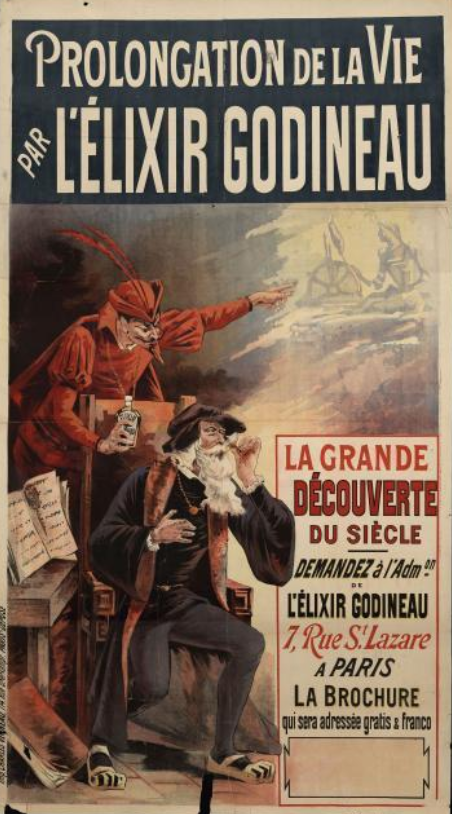
\includegraphics[width=0.7\textwidth]{images/brev77.png}
\end{center}
\breakpage